\section{Prospetto economico}
	\subsection{Analisi}
	Nel periodo riguardante la fase di Analisi le ore tra i ruoli sono state divise nel seguente modo: \\
	\begin{figure}[H]
		\centering
		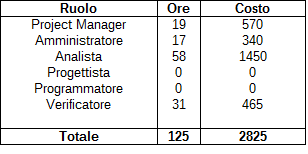
\includegraphics[scale=0.75]{immagini/tabelle/analisi-costo.png}
		\caption{Costo per ruolo, fase di Analisi}
	\end{figure}
	I seguenti grafici illustrano rispettivamente come ciascun ruolo abbia influito sul totale
delle ore e dei costi della fase di Analisi. \\
	\begin{figure}[H]
		\centering
		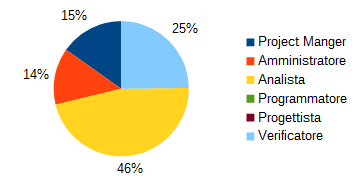
\includegraphics[scale=1]{immagini/grafici/analisi-torta.png}
		\caption{Ore per ruoli, fase di Analisi}
	\end{figure}
	\begin{figure}[H]
		\centering
		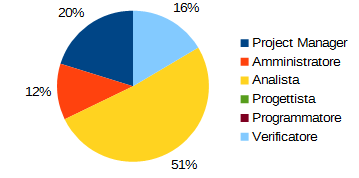
\includegraphics[scale=1]{immagini/grafici/analisi-torta-costo.png}
		\caption{Costi per ruoli, fase di Analisi}
	\end{figure}
	\subsection{Analisi di Dettaglio}
	Nel periodo riguardante la fase di Analisi di Dettaglio le ore tra i ruoli sono state divise nel seguente modo: \\
	\begin{figure}[H]
		\centering
		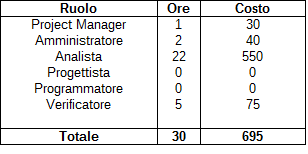
\includegraphics[scale=0.75]{immagini/tabelle/analisi_dettaglio-costo.png}
		\caption{Costo per ruolo, fase di Analisi di Dettaglio}
	\end{figure}
	I seguenti grafici illustrano rispettivamente come ciascun ruolo abbia influito sul totale
delle ore e dei costi della fase di Analisi di Dettaglio. \\
	\begin{figure}[H]
		\centering
		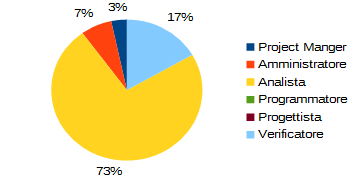
\includegraphics[scale=1]{immagini/grafici/analisi_dettaglio-torta.png}
		\caption{Ore per ruoli, fase di Analisi di Dettaglio}
	\end{figure}
	\begin{figure}[H]
		\centering
		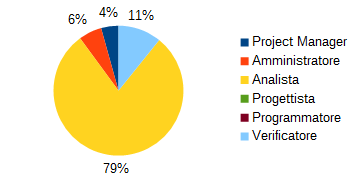
\includegraphics[scale=1]{immagini/grafici/analisi_dettaglio-torta-costo.png}
		\caption{Costi per ruoli, fase di Analisi di Dettaglio}
	\end{figure}
	\subsection{Progettazione Architetturale}
	Nel periodo riguardante la fase di Progettazione Architetturale le ore tra i ruoli sono state divise nel seguente modo: \\
	\begin{figure}[H]
		\centering
		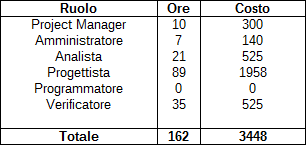
\includegraphics[scale=0.75]{immagini/tabelle/progettazione_architetturale-costo.png}
		\caption{Costo per ruolo, fase di Progettazione Architetturale}
	\end{figure}
	I seguenti grafici illustrano rispettivamente come ciascun ruolo abbia influito sul totale
delle ore e dei costi della fase di Progettazione Architetturale. \\
	\begin{figure}[H]
		\centering
		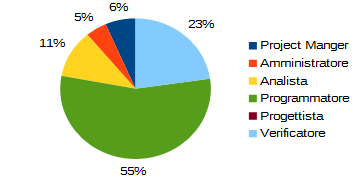
\includegraphics[scale=1]{immagini/grafici/progettazione_architetturale-torta.png}
		\caption{Ore per ruoli, fase di Progettazione Architetturale}
	\end{figure}
	\begin{figure}[H]
		\centering
		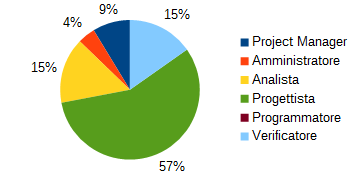
\includegraphics[scale=1]{immagini/grafici/progettazione_architetturale-torta-costo.png}
		\caption{Costi per ruoli, fase di Progettazione Architetturale}
	\end{figure}
	\subsection{Progettazione di Dettaglio e Codifica}
	Nel periodo riguardante la fase di Progettazione di Dettaglio e Codifica le ore tra i ruoli sono state divise nel seguente modo: \\
	\begin{figure}[H]
		\centering
		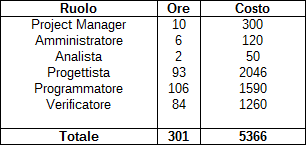
\includegraphics[scale=0.75]{immagini/tabelle/progettazione_dettaglio_codifica-costo.png}
		\caption{Costo per ruolo, fase di Progettazione di Dettaglio e Codifica}
	\end{figure}
	I seguenti grafici illustrano rispettivamente come ciascun ruolo abbia influito sul totale
delle ore e dei costi della fase di Progettazione di Dettaglio e Codifica. \\
	\begin{figure}[H]
		\centering
		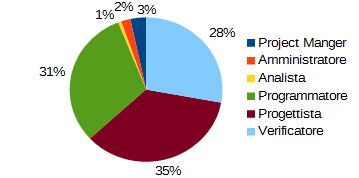
\includegraphics[scale=1]{immagini/grafici/progettazione_dettaglio_codifica-torta.png}
		\caption{Ore per ruoli, fase di Progettazione di Dettaglio e Codifica}
	\end{figure}
	\begin{figure}[H]
		\centering
		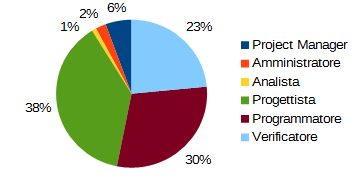
\includegraphics[scale=1]{immagini/grafici/progettazione_dettaglio_codifica-torta-costo.png}
		\caption{Costi per ruoli, fase di Progettazione di Dettaglio e Codifica}
	\end{figure}
	\subsection{Verifica e Validazione}
	Nel periodo riguardante la fase di Verifica e Validazione le ore tra i ruoli sono state divise nel seguente modo: \\
	\begin{figure}[H]
		\centering
		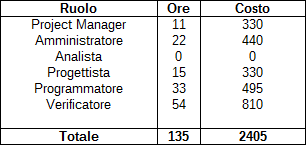
\includegraphics[scale=0.75]{immagini/tabelle/validazione-costo.png}
		\caption{Costo per ruolo, fase di Verifica e Validazione}
	\end{figure}
	I seguenti grafici illustrano rispettivamente come ciascun ruolo abbia influito sul totale
delle ore e dei costi della fase di Verifica e Validazione. \\
	\begin{figure}[H]
		\centering
		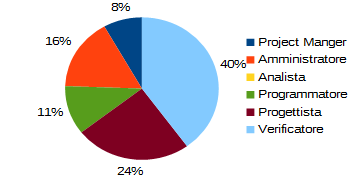
\includegraphics[scale=1]{immagini/grafici/validazione-torta.png}
		\caption{Ore per ruoli, fase di Verifica e Validazione}
	\end{figure}
	\begin{figure}[H]
		\centering
		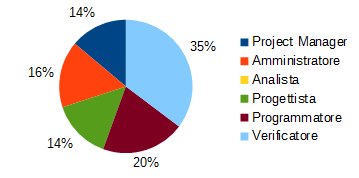
\includegraphics[scale=1]{immagini/grafici/validazione-torta-costo.png}
		\caption{Costi per ruoli, fase di Verifica e Validazione}
	\end{figure}
	\subsection{Totale}
		\subsubsection{Ore totali con investimento}
		Le ore totali, previste per la realizzazione dell'intero progetto, comprese le ore di investimento, sono riportate nella tabella seguente. \\
		\begin{figure}[H]
			\centering
			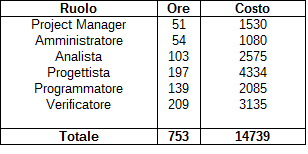
\includegraphics[scale=0.75]{immagini/tabelle/riepilogo_conclusivo-costo.png}
			\caption{Costo totale per ruolo}
		\end{figure}
		I seguenti grafici illustrano rispettivamente come ciascun ruolo abbia influito sul totale delle ore e dei costi di tutto il progetto compresa la fase di investimento. \\
		\begin{figure}[H]
		\centering
			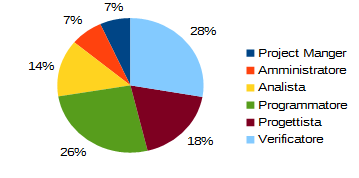
\includegraphics[scale=1]{immagini/grafici/riepilogo_conclusivo-torta.png}
			\caption{Ore totali per ruoli}
		\end{figure}
		\begin{figure}[H]
			\centering
			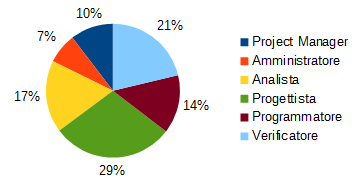
\includegraphics[scale=1]{immagini/grafici/riepilogo_conclusivo-torta-costo.png}
			\caption{Costi totali per ruoli}
		\end{figure}
		\subsubsection{Ore rendicontate}
		Le ore totali rendicontate sono riportate nella tabella sottostante, insieme al costo totale del progetto a carico del committente. \\
		\begin{figure}[H]
			\centering
			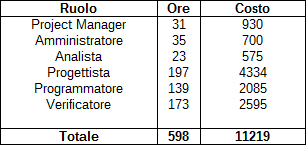
\includegraphics[scale=0.75]{immagini/tabelle/orario_rendicontato-costo.png}
			\caption{Costo totale retribuito per ruolo}
		\end{figure}
		I seguenti grafici illustrano rispettivamente come ciascun ruolo abbia influito sul totale delle ore e dei costi retribuiti. \\
		\begin{figure}[H]
		\centering
			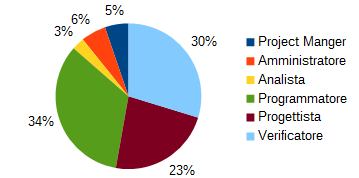
\includegraphics[scale=1]{immagini/grafici/orario_rendicontato-torta.png}
			\caption{Ore totali retribuite per ruoli}
		\end{figure}
		\begin{figure}[H]
			\centering
			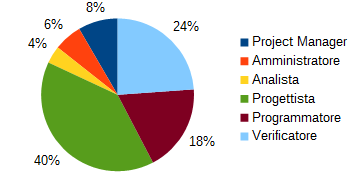
\includegraphics[scale=1]{immagini/grafici/orario_rendicontato-torta-costo.png}
			\caption{Costi totali retribuiti per ruoli}
		\end{figure}
		\subsubsection{Conclusioni}